%
% Template for DAS course projects
%
\documentclass[a4paper,11pt,oneside]{book}
\usepackage[latin1]{inputenc}
\usepackage[english]{babel}
\usepackage{amsfonts}
\usepackage{amsmath}
\usepackage{amssymb,amsmath,color}
\usepackage{cite}
\usepackage{graphicx}
\usepackage{float}
\usepackage{caption}
\usepackage{subcaption}

\begin{document}
\pagestyle{myheadings}

%%%%%%%%%%% Cover %%%%%%%%%%%
\thispagestyle{empty}                                                 
\begin{center}                                                            
    \vspace{5mm}
    {\LARGE UNIVERSIT\`A DI BOLOGNA} \\                       
      \vspace{5mm}
\end{center}
\begin{center}
  
\includegraphics[scale=.27]{figs/logo_unibo}
\end{center}
\begin{center}
      \vspace{5mm}
      {\LARGE School of Engineering} \\
        \vspace{3mm}
      {\Large Master Degree in Automation Engineering} \\
      \vspace{20mm}
      {\LARGE Distributed Autonomous Systems} \\
      \vspace{5mm}{\Large\textbf{TITLE}}                  
      \vspace{15mm}
\end{center}
\begin{minipage}{0.48\linewidth}
      \raggedright
     {\large Professors:}\\
     \textbf{Giuseppe Notarstefano} \\
     \textbf{Ivano Notarnicola} \\        
%      \vspace{13mm}
\end{minipage}
\begin{minipage}{0.48\linewidth}
      \raggedleft
      {\large Students:}\\
      \textbf{\@ Valerio Costa} \\
      \textbf{\@ Tian Cheng Xia} \\  
\end{minipage}
\begin{center}
\vfill
      {\large Academic year \@2024/2025} \\
\end{center}



\newpage
\thispagestyle{empty}

%%%%%%%%%%% Abstract %%%%%%%%%%%%
\begin{center}
\chapter*{}
\thispagestyle{empty}
{\Huge \textbf{Abstract}}\\
\vspace{15mm}
\end{center}

\tableofcontents \thispagestyle{empty}
% \listoffigures\thispagestyle{empty}

%%%%%%%%%% Introduction %%%%%%%%%%
\chapter*{Introduction}
\addcontentsline{toc}{chapter}{Introduction}
\section*{Motivations} 

\section*{Contributions}


\chapter{Multi-Robot Target Localization}

\section{Gradient tracking with quadratic functions}


\subsection{Different graph patterns comparison}

\begin{figure}[H]
      \centering
      \begin{subfigure}[t]{0.49\textwidth}
            \centering
            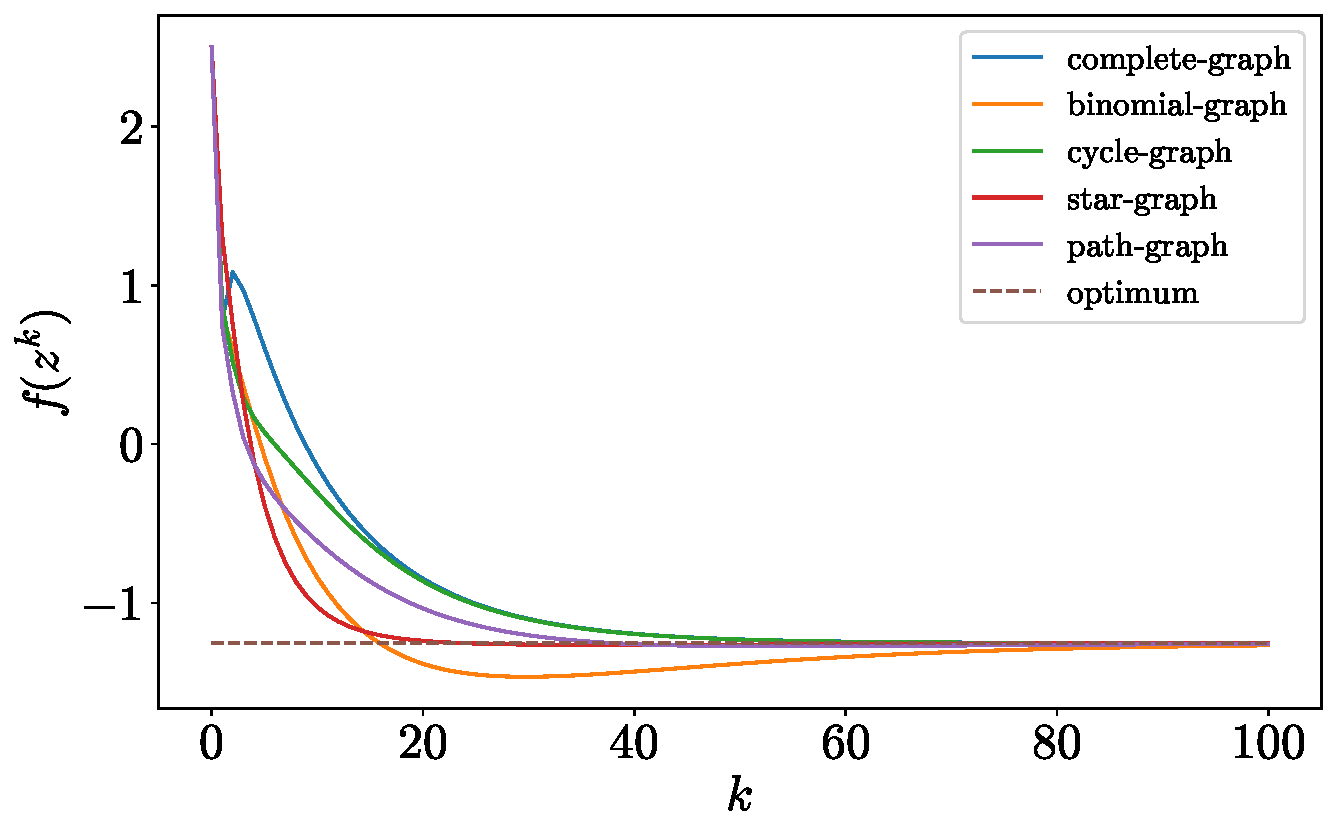
\includegraphics[width=\linewidth]{./figs/quadratic/cost_5_3_100.pdf} 
            \caption{Cost evolution}
      \end{subfigure}
      \hfill
      \begin{subfigure}[t]{0.49\textwidth}
            \centering
            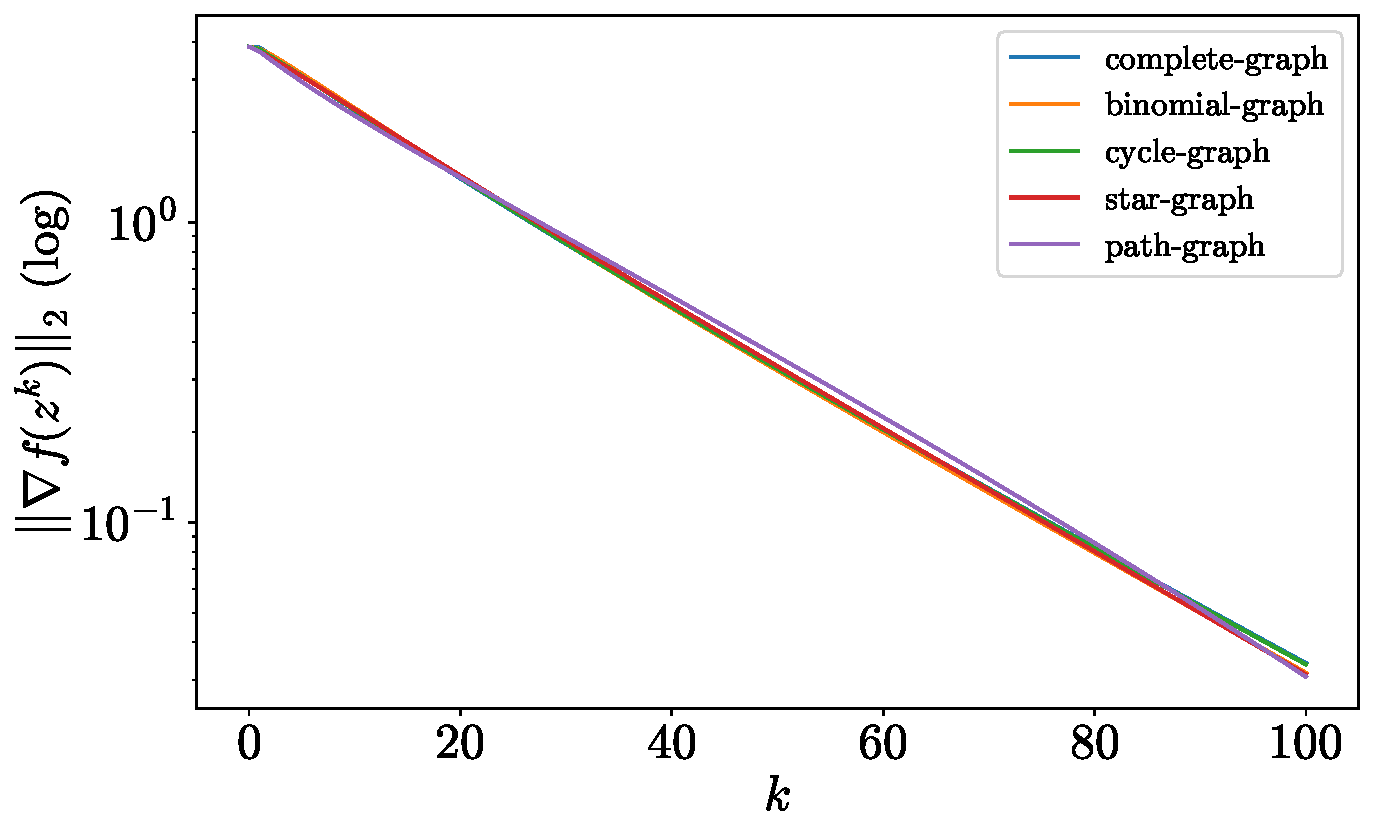
\includegraphics[width=\linewidth]{./figs/quadratic/gradient_5_3_100.pdf} 
            \caption{Gradient norm evolution}
      \end{subfigure}
      \hfill
      \begin{subfigure}[t]{0.49\textwidth}
            \centering
            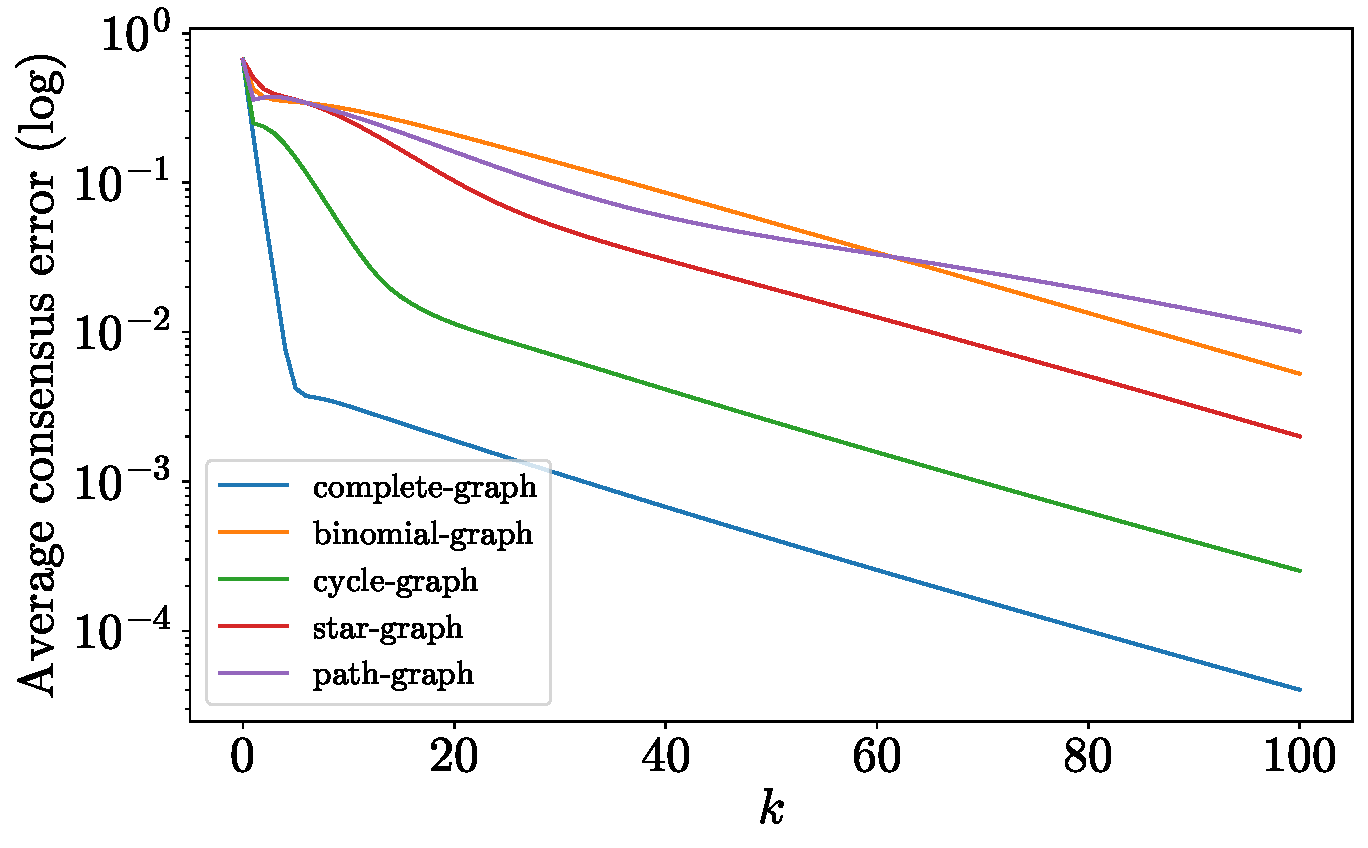
\includegraphics[width=\linewidth]{./figs/quadratic/consensus_5_3_100.pdf} 
            \caption{Consensus error}
      \end{subfigure}
      \caption{Configuration with $5$ agents in $\mathbb{R}^{3}$}
\end{figure}

\begin{figure}[H]
      \centering
      \begin{subfigure}[t]{0.49\textwidth}
            \centering
            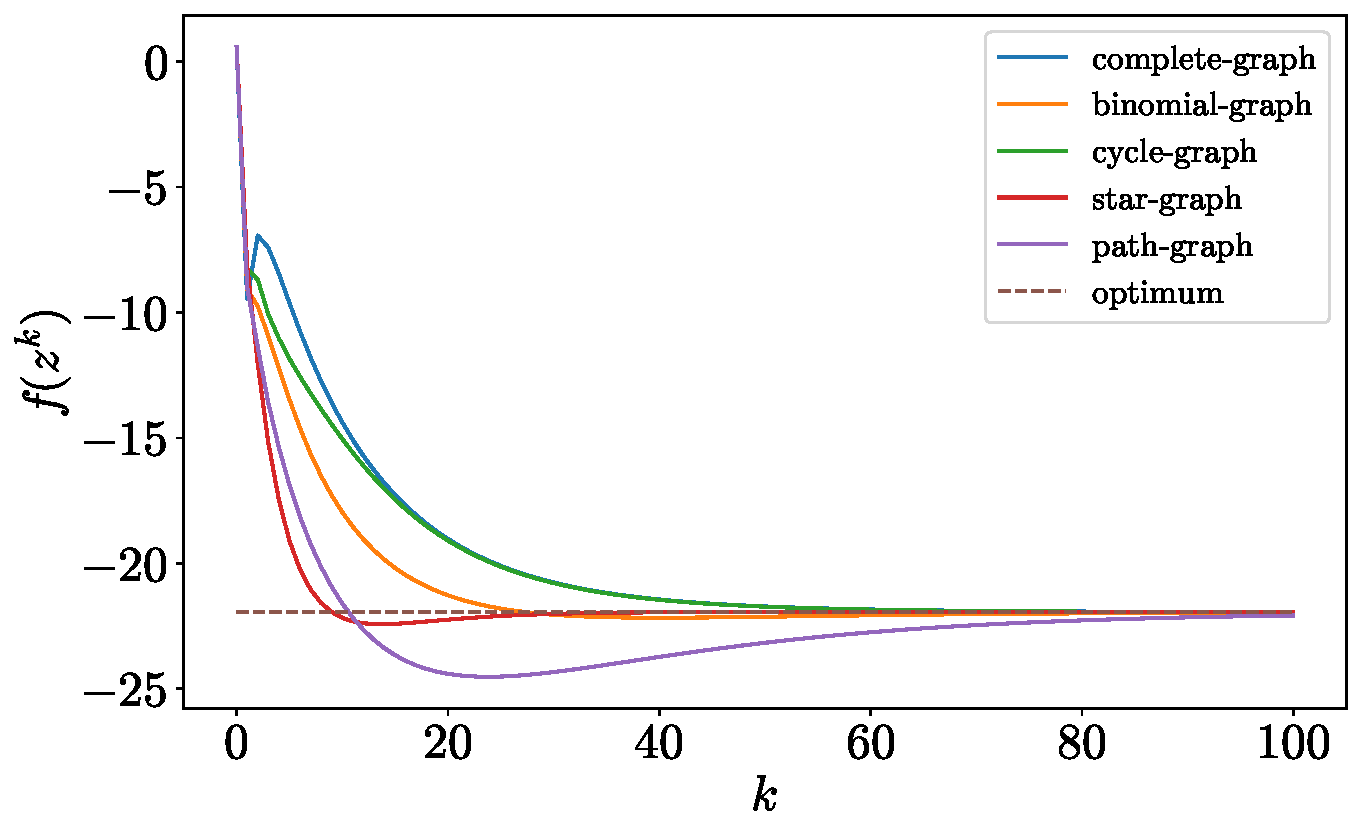
\includegraphics[width=\linewidth]{./figs/quadratic/cost_5_15_100.pdf} 
            \caption{Cost evolution}
      \end{subfigure}
      \hfill
      \begin{subfigure}[t]{0.49\textwidth}
            \centering
            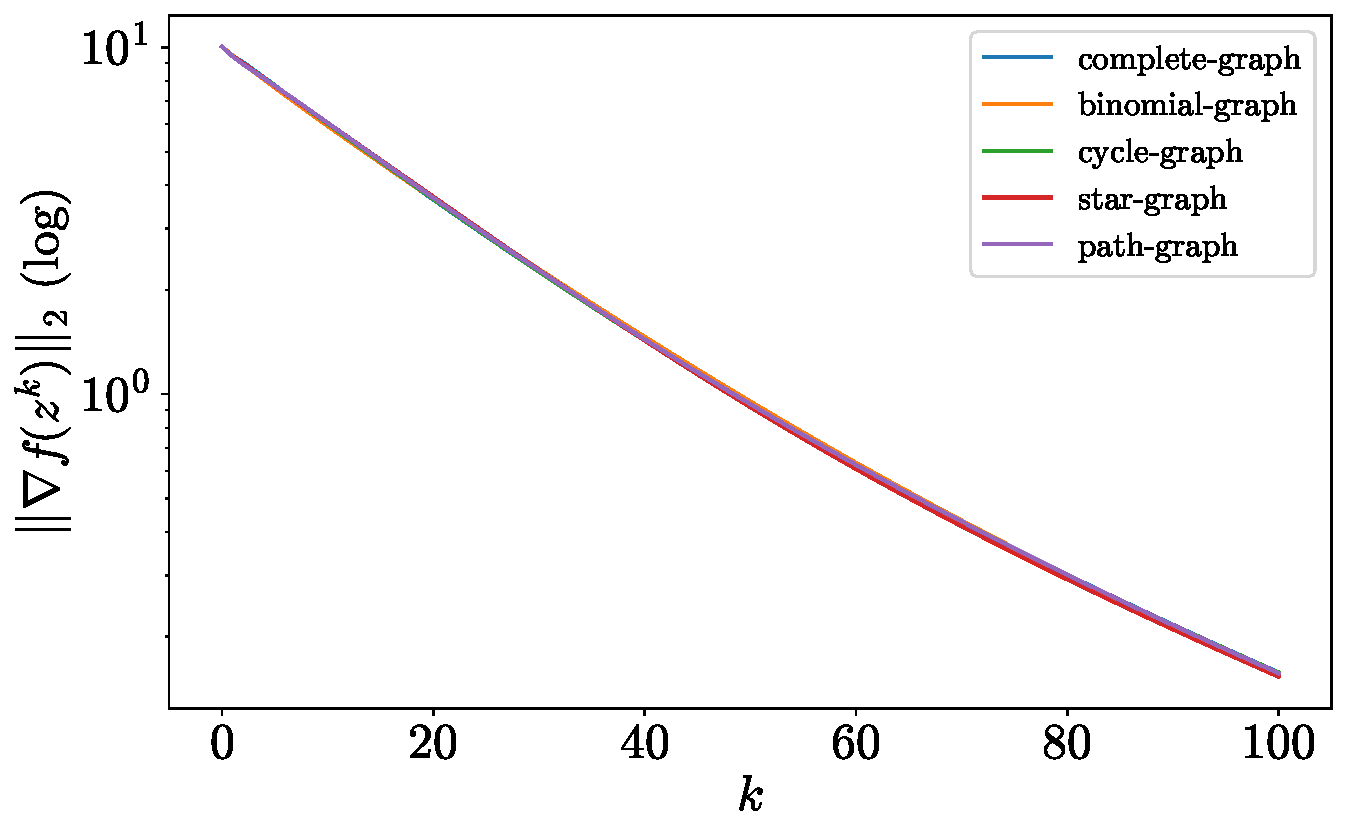
\includegraphics[width=\linewidth]{./figs/quadratic/gradient_5_15_100.pdf} 
            \caption{Gradient norm evolution}
      \end{subfigure}
      % \hfill
      % \begin{subfigure}[t]{0.49\textwidth}
      %       \centering
      %       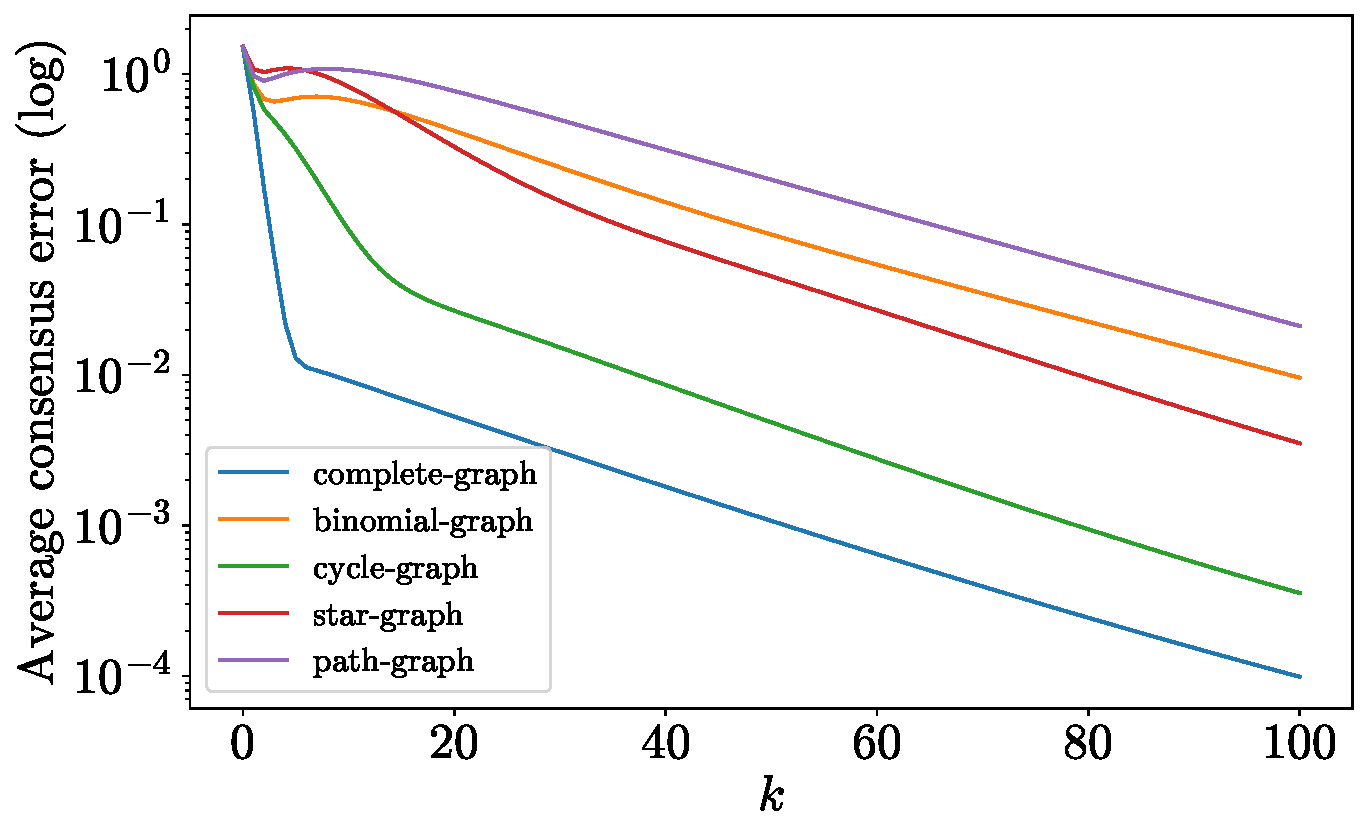
\includegraphics[width=\linewidth]{./figs/quadratic/consensus_5_15_100.pdf} 
      %       \caption{Consensus error}
      % \end{subfigure}
      \caption{Configuration with $5$ agents in $\mathbb{R}^{15}$}
\end{figure}

\begin{figure}[H]
      \centering
      \begin{subfigure}[t]{0.49\textwidth}
            \centering
            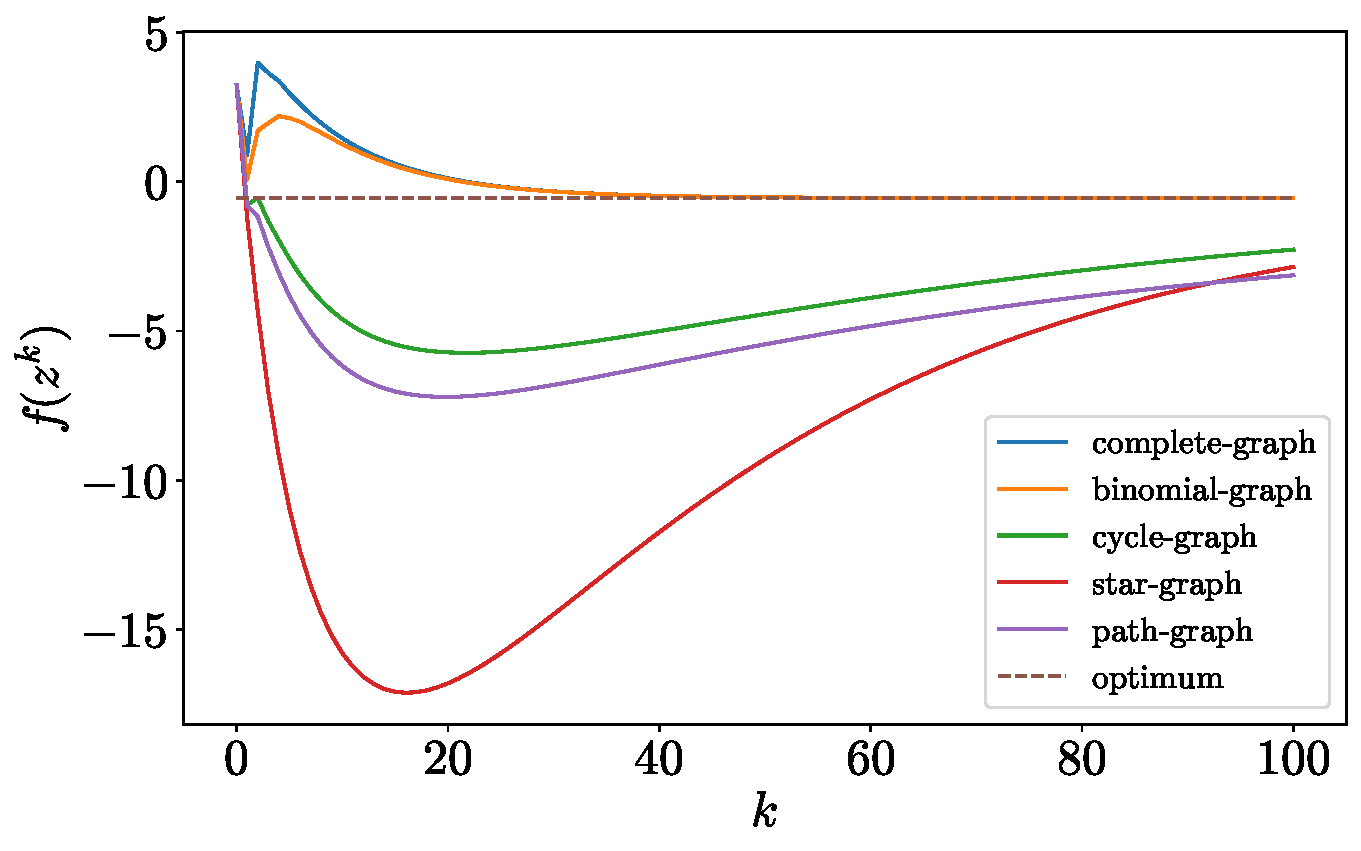
\includegraphics[width=\linewidth]{./figs/quadratic/cost_15_3_100.pdf} 
            \caption{Cost evolution}
      \end{subfigure}
      \hfill
      \begin{subfigure}[t]{0.49\textwidth}
            \centering
            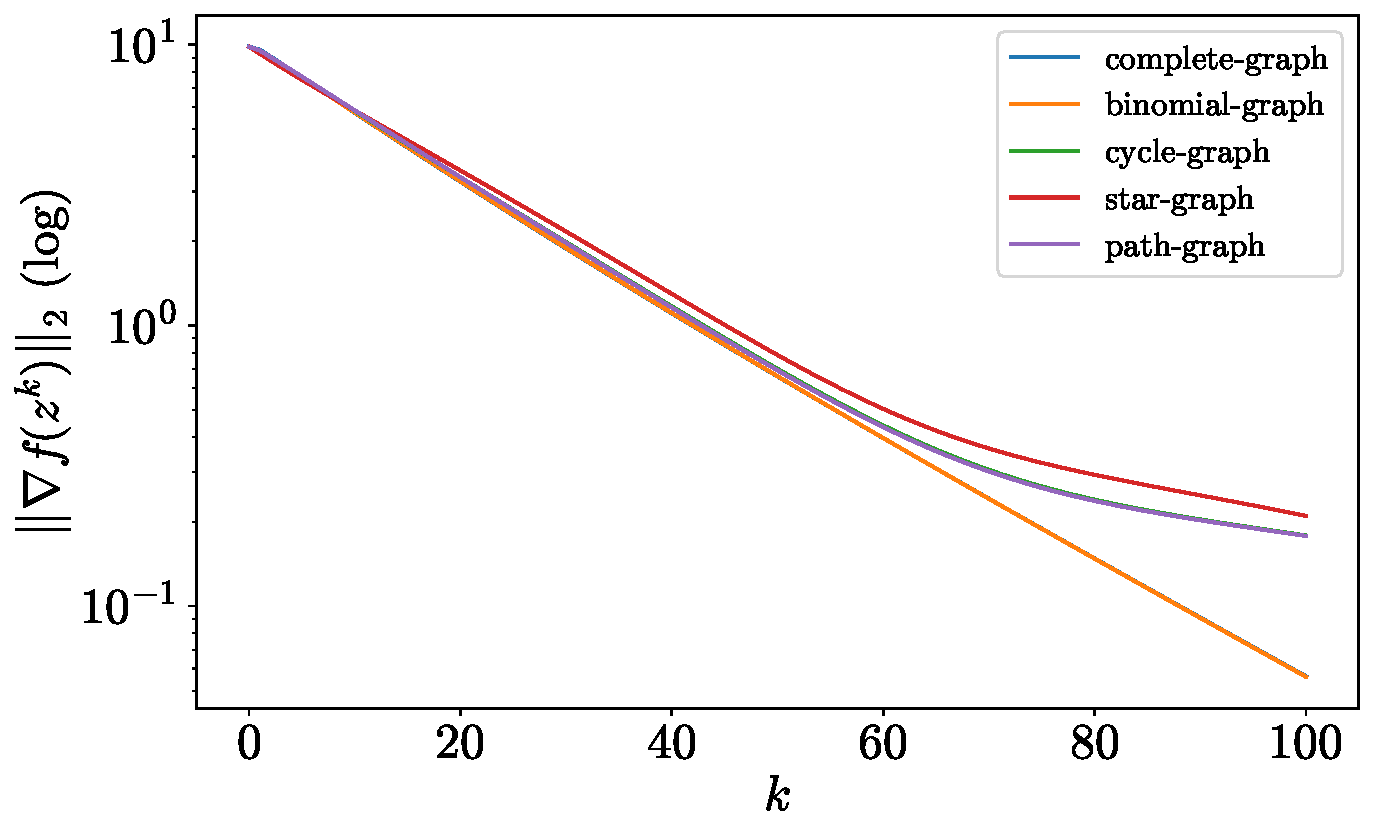
\includegraphics[width=\linewidth]{./figs/quadratic/gradient_15_3_100.pdf} 
            \caption{Gradient norm evolution}
      \end{subfigure}
      % \hfill
      % \begin{subfigure}[t]{0.49\textwidth}
      %       \centering
      %       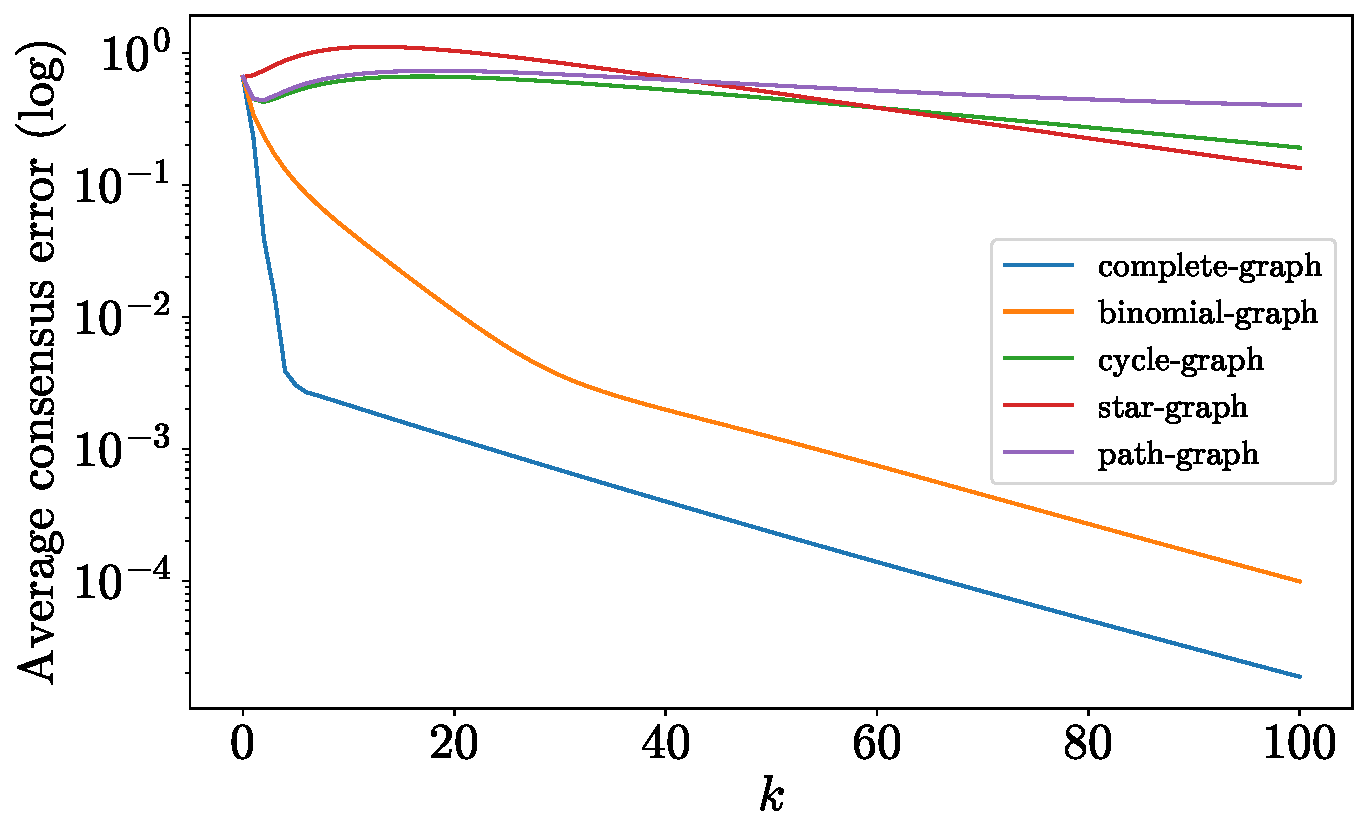
\includegraphics[width=\linewidth]{./figs/quadratic/consensus_15_3_100.pdf} 
      %       \caption{Consensus error}
      % \end{subfigure}
      \caption{Configuration with $15$ agents in $\mathbb{R}^{3}$}
\end{figure}

\begin{figure}[H]
      \centering
      \begin{subfigure}[t]{0.49\textwidth}
            \centering
            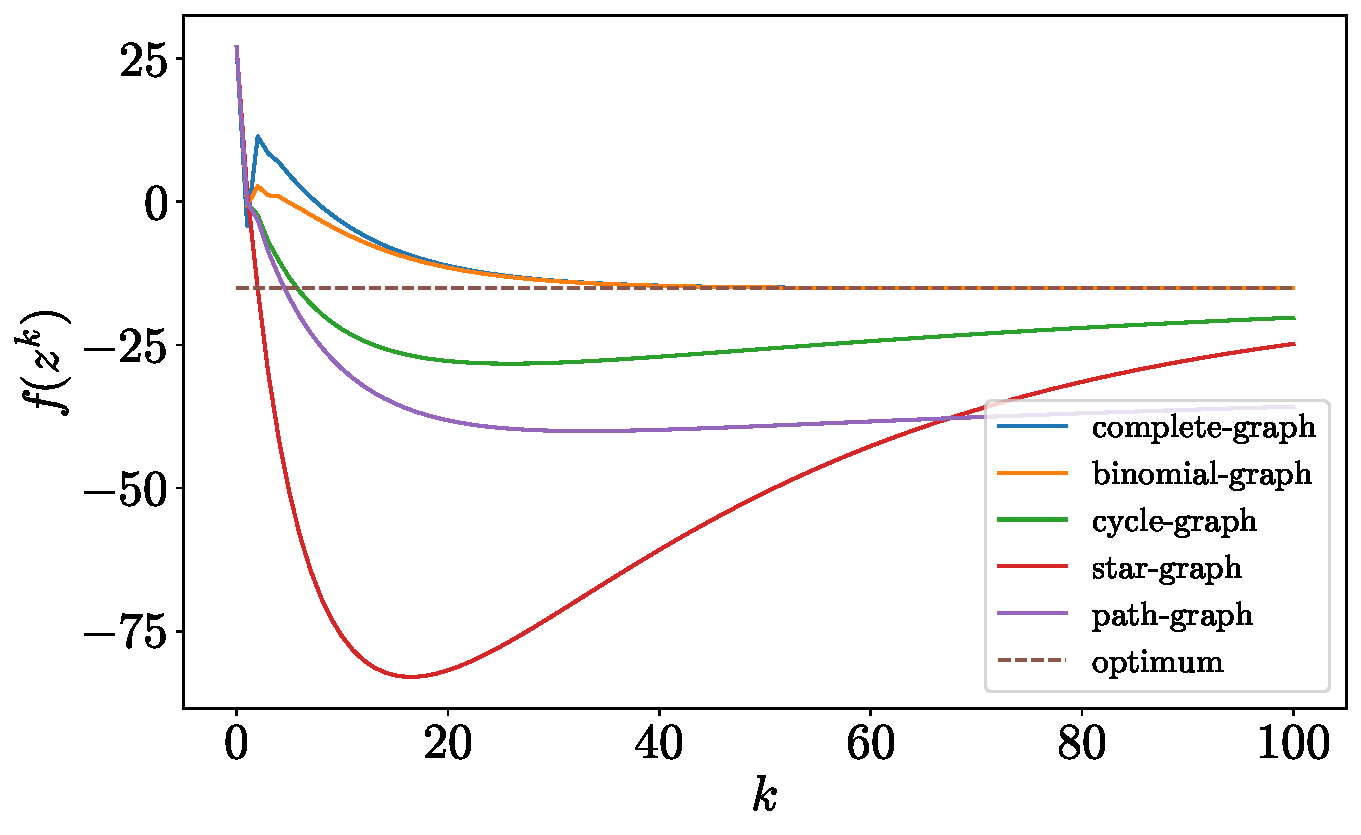
\includegraphics[width=\linewidth]{./figs/quadratic/cost_15_15_100.pdf} 
            \caption{Cost evolution}
      \end{subfigure}
      \hfill
      \begin{subfigure}[t]{0.49\textwidth}
            \centering
            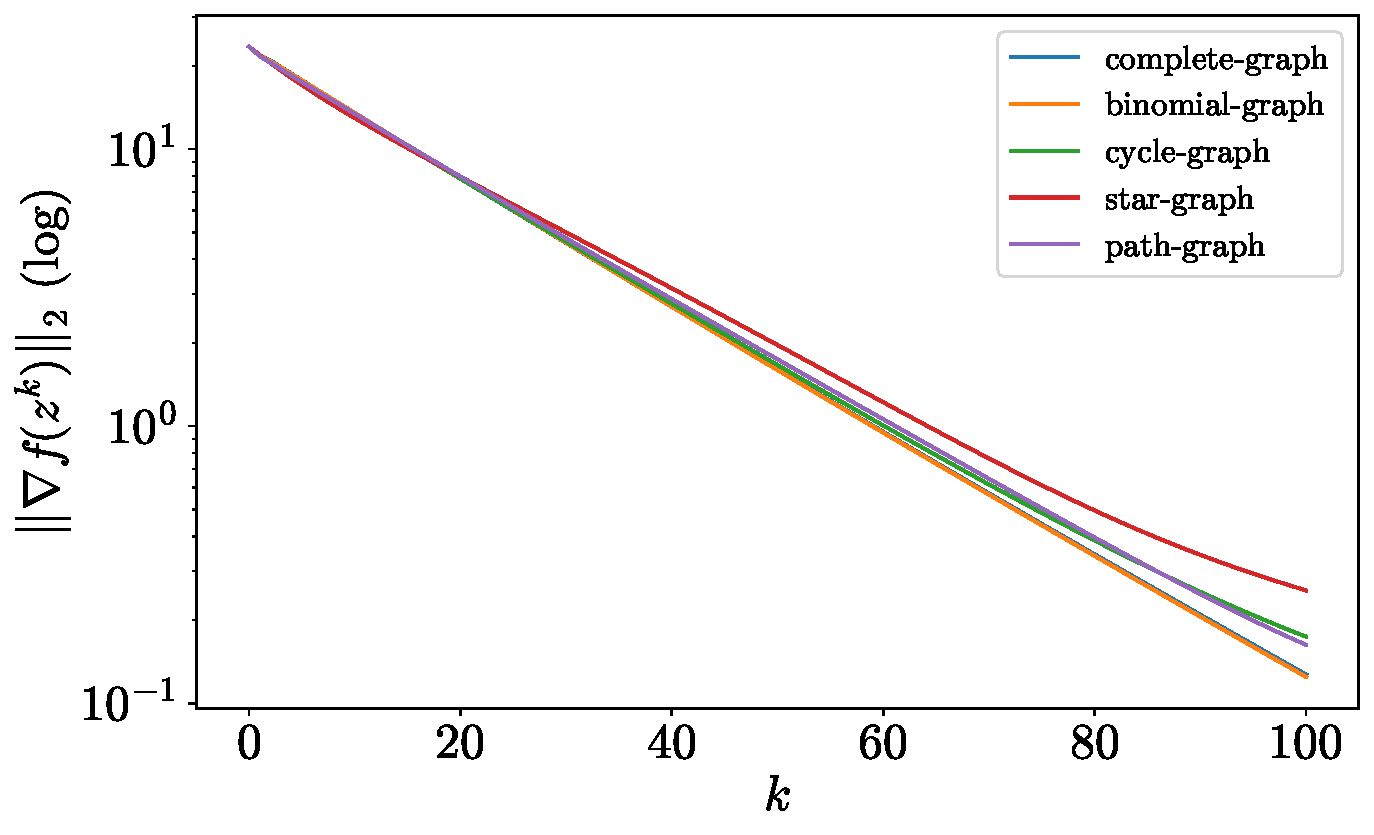
\includegraphics[width=\linewidth]{./figs/quadratic/gradient_15_15_100.pdf} 
            \caption{Gradient norm evolution}
      \end{subfigure}
      % \hfill
      % \begin{subfigure}[t]{0.49\textwidth}
      %       \centering
      %       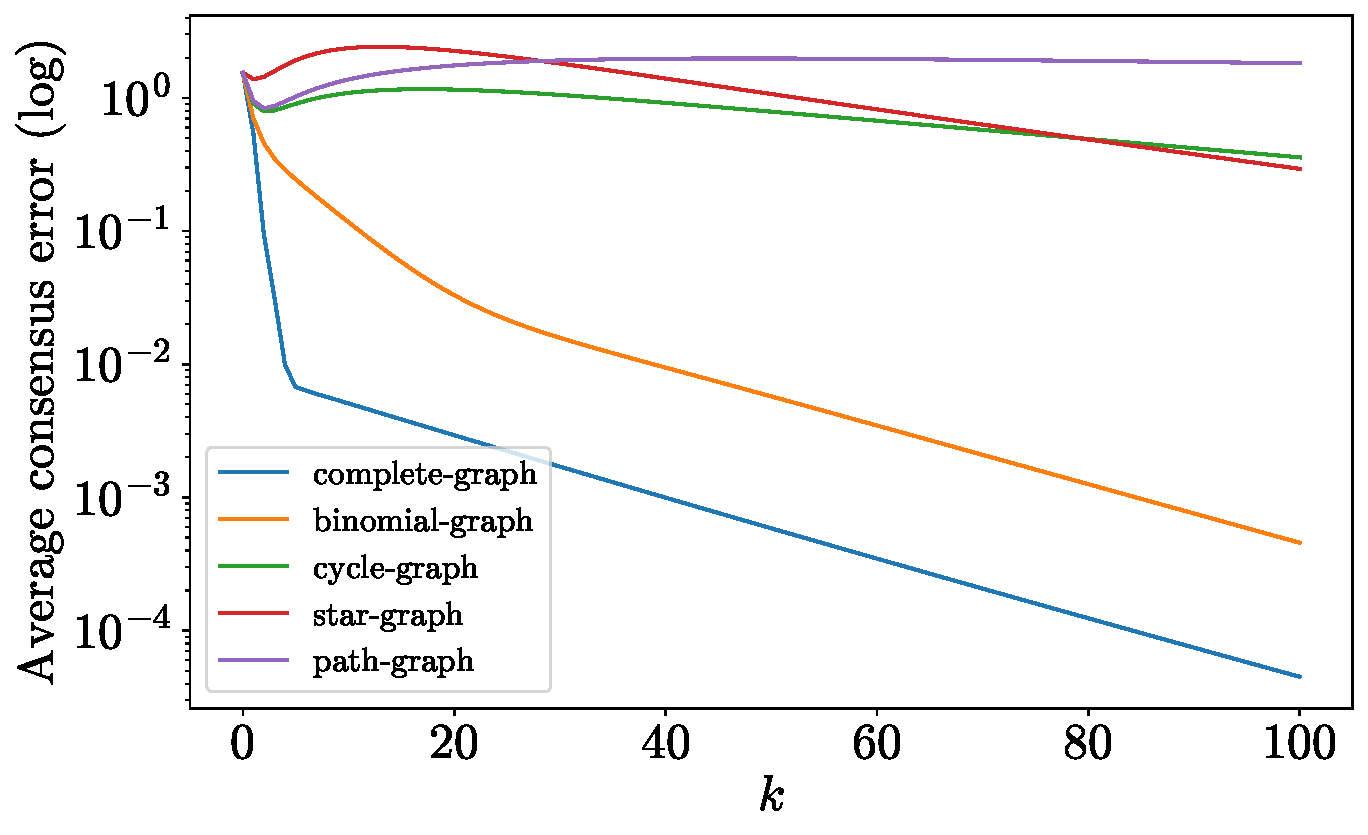
\includegraphics[width=\linewidth]{./figs/quadratic/consensus_15_15_100.pdf} 
      %       \caption{Consensus error}
      % \end{subfigure}
      \caption{Configuration with $15$ agents in $\mathbb{R}^{15}$}
\end{figure}



\begin{figure}[H]
      \centering
      \begin{subfigure}[t]{0.49\textwidth}
            \centering
            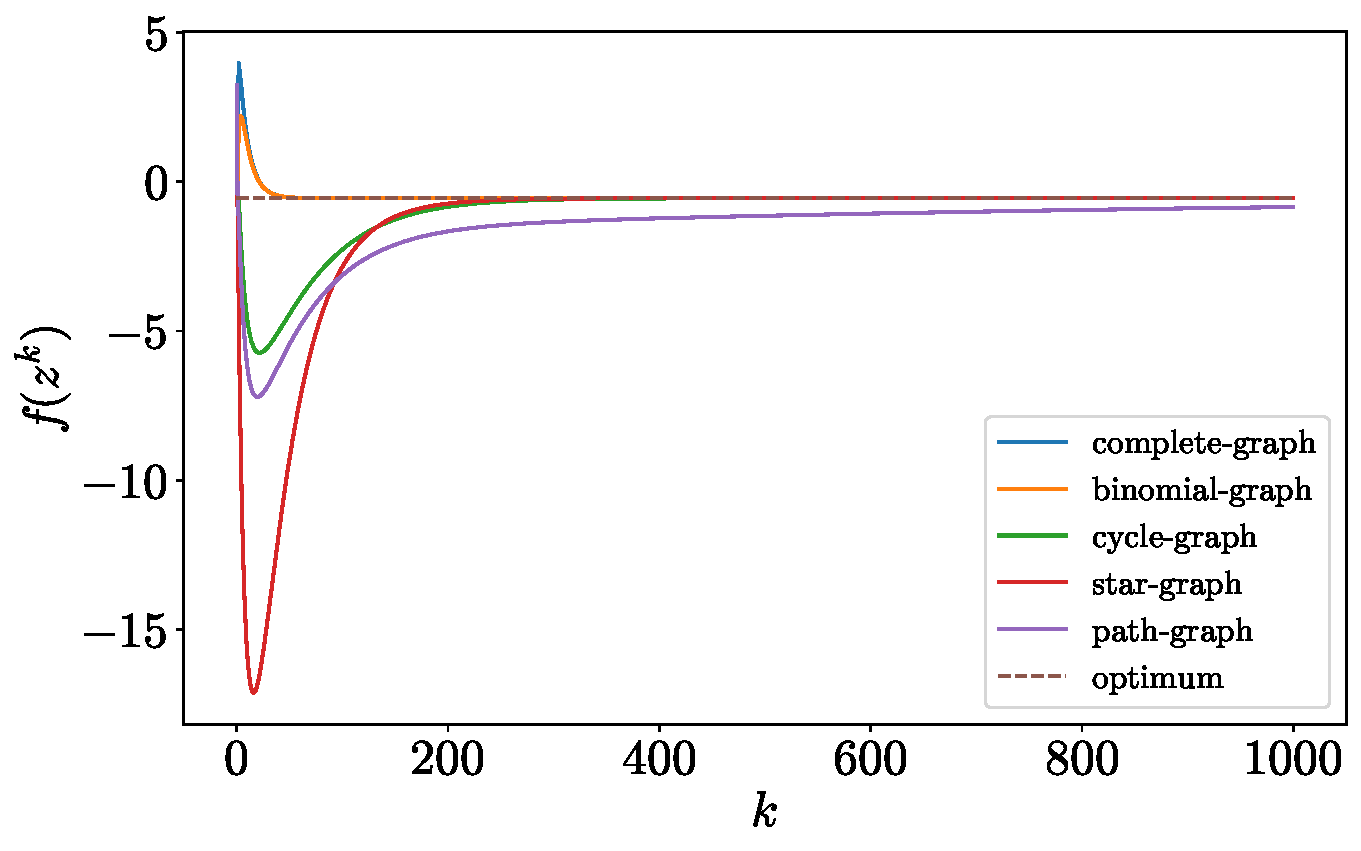
\includegraphics[width=\linewidth]{./figs/quadratic/cost_15_3_1000.pdf} 
            \caption{Cost evolution}
      \end{subfigure}
      \hfill
      \begin{subfigure}[t]{0.49\textwidth}
            \centering
            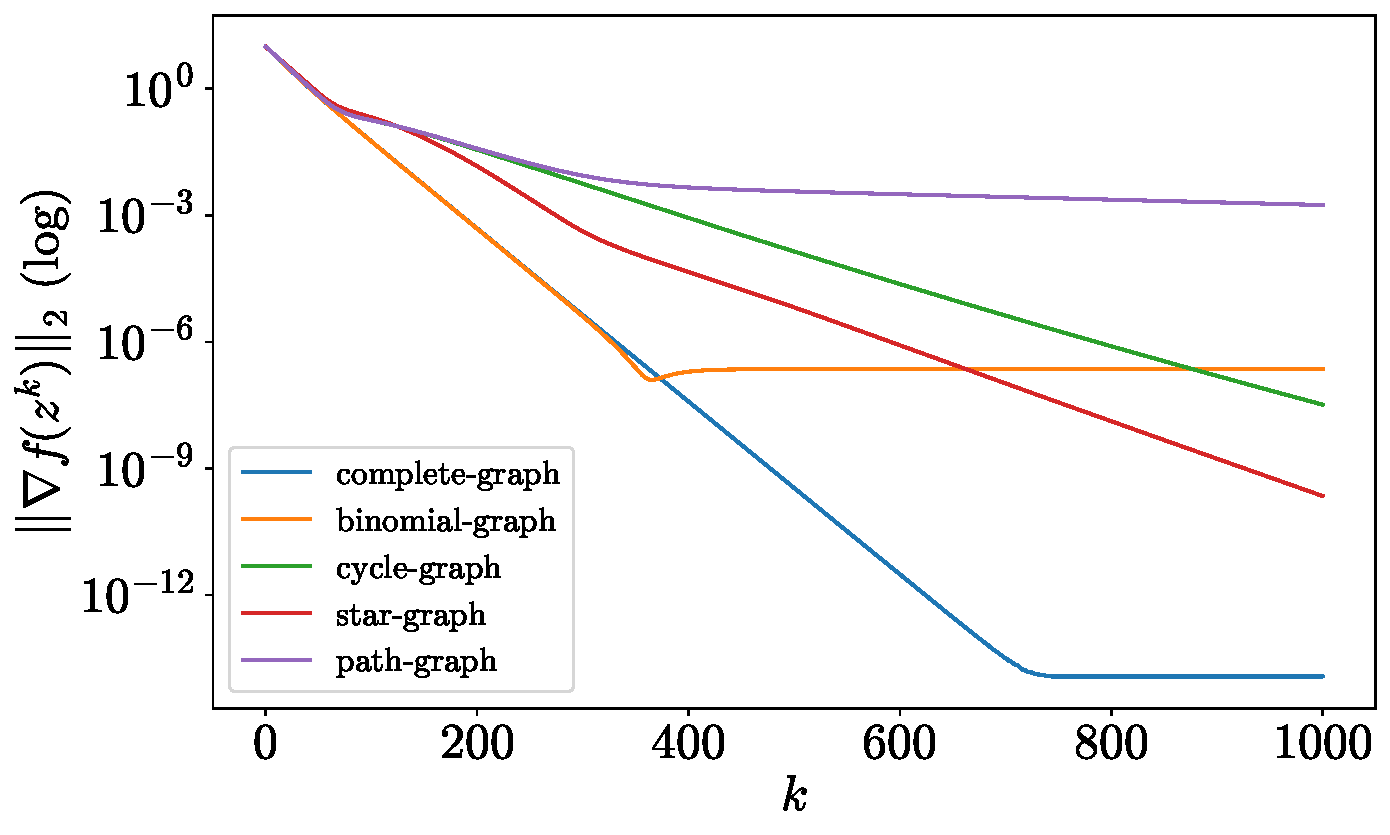
\includegraphics[width=\linewidth]{./figs/quadratic/gradient_15_3_1000.pdf} 
            \caption{Gradient norm evolution}
      \end{subfigure}
      % \hfill
      % \begin{subfigure}[t]{0.49\textwidth}
      %       \centering
      %       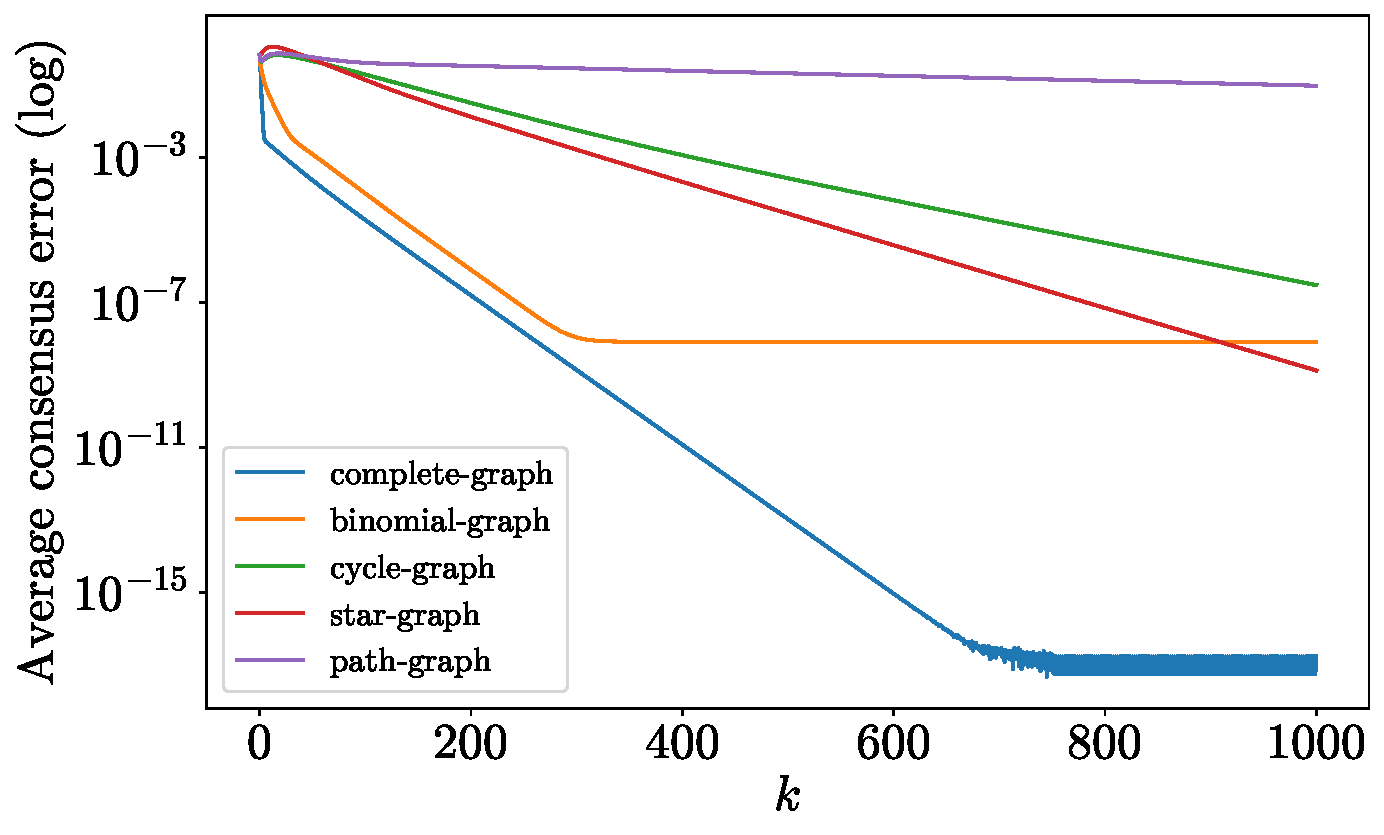
\includegraphics[width=\linewidth]{./figs/quadratic/consensus_15_3_1000.pdf} 
      %       \caption{Consensus error}
      % \end{subfigure}
      \caption{Configuration with $15$ agents in $\mathbb{R}^{3}$ to convergence}
\end{figure}


\subsection{Comparison with centralized gradient}

\begin{figure}[H]
      \centering
      \begin{subfigure}[t]{0.49\textwidth}
            \centering
            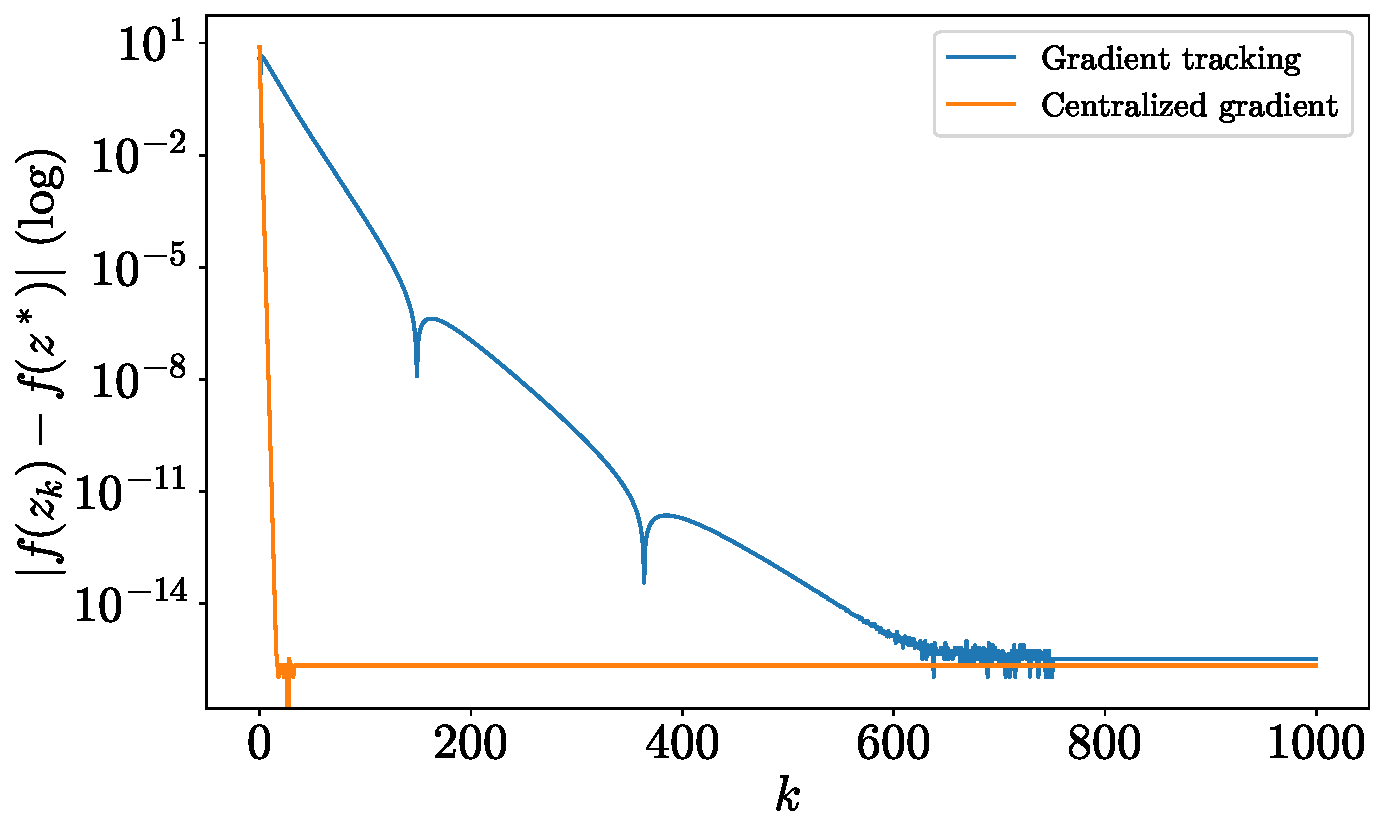
\includegraphics[width=\linewidth]{./figs/quadratic/distance_centralized_15_3_1000.pdf} 
            \caption{Distance to optimum}
      \end{subfigure}
      \hfill
      \begin{subfigure}[t]{0.49\textwidth}
            \centering
            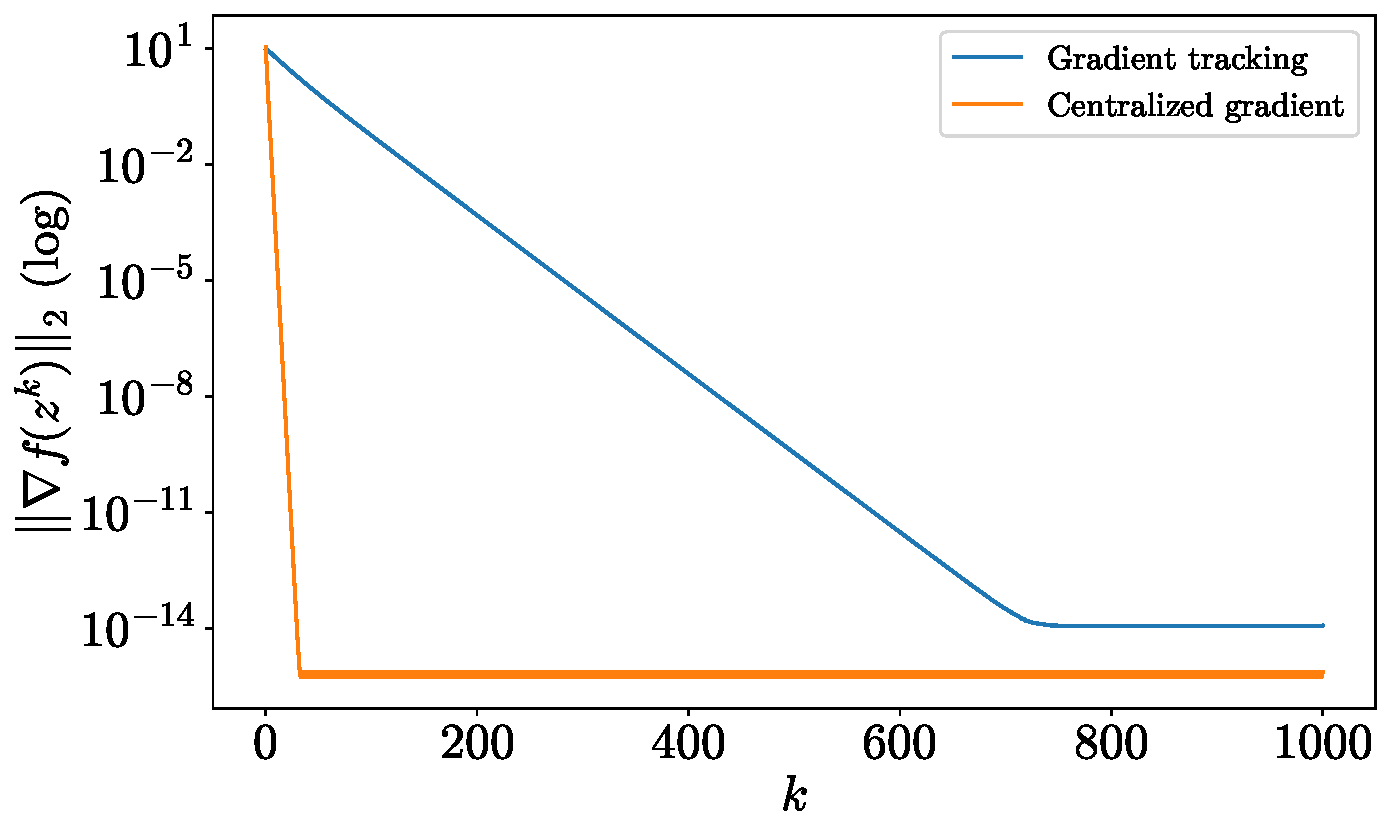
\includegraphics[width=\linewidth]{./figs/quadratic/gradient_centralized_15_3_1000.pdf} 
            \caption{Gradient norm evolution}
      \end{subfigure}
      \caption{Configuration with $15$ agents in $\mathbb{R}^{3}$ compared to centralized gradient}
\end{figure}


\section{Cooperative multi-robot target localization}

\subsection{Different graph patterns comparison}

\begin{figure}[H]
      \centering
      \begin{subfigure}[t]{0.49\textwidth}
            \centering
            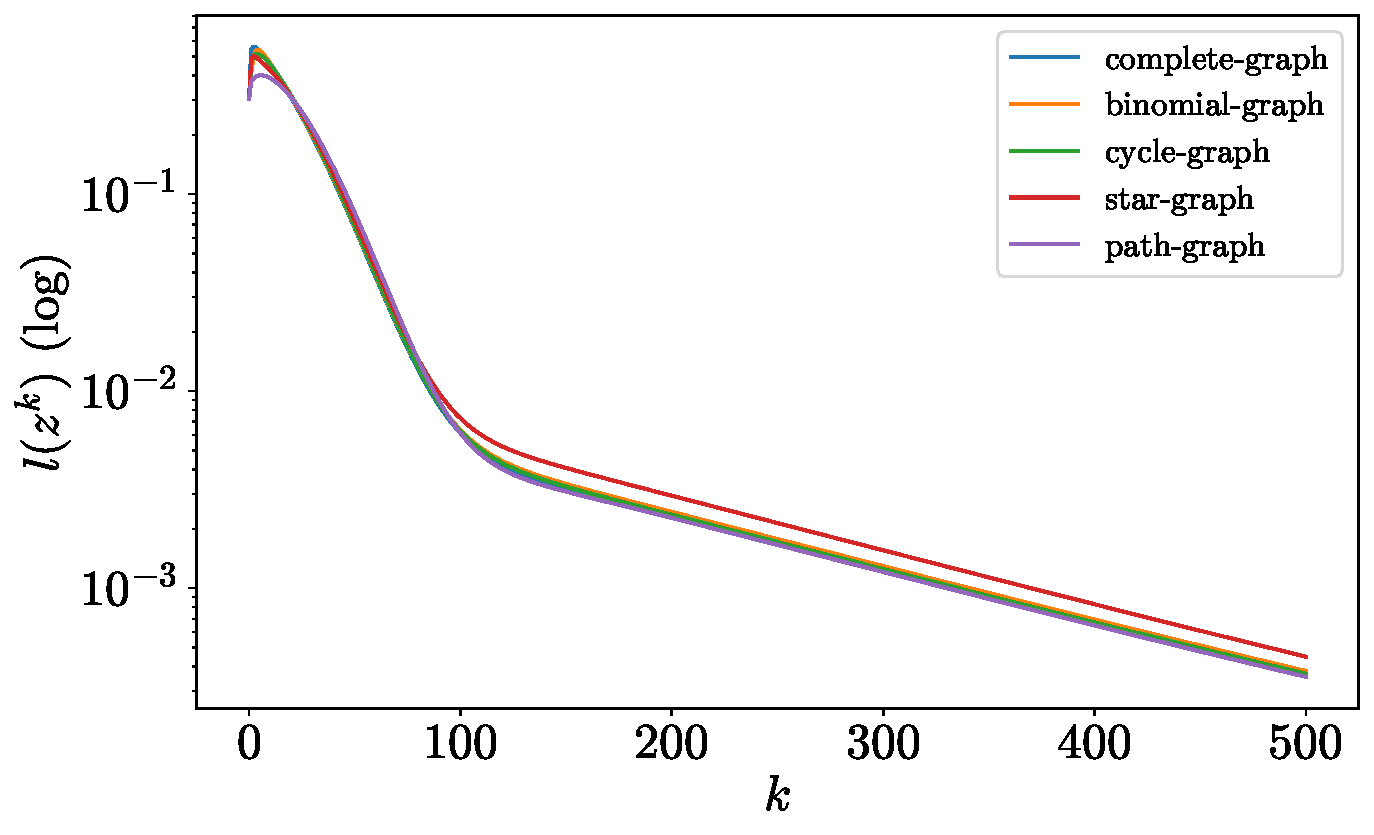
\includegraphics[width=\linewidth]{./figs/tracking/loss_5_1_2_500.pdf} 
            \caption{Loss evolution}
      \end{subfigure}
      \hfill
      \begin{subfigure}[t]{0.49\textwidth}
            \centering
            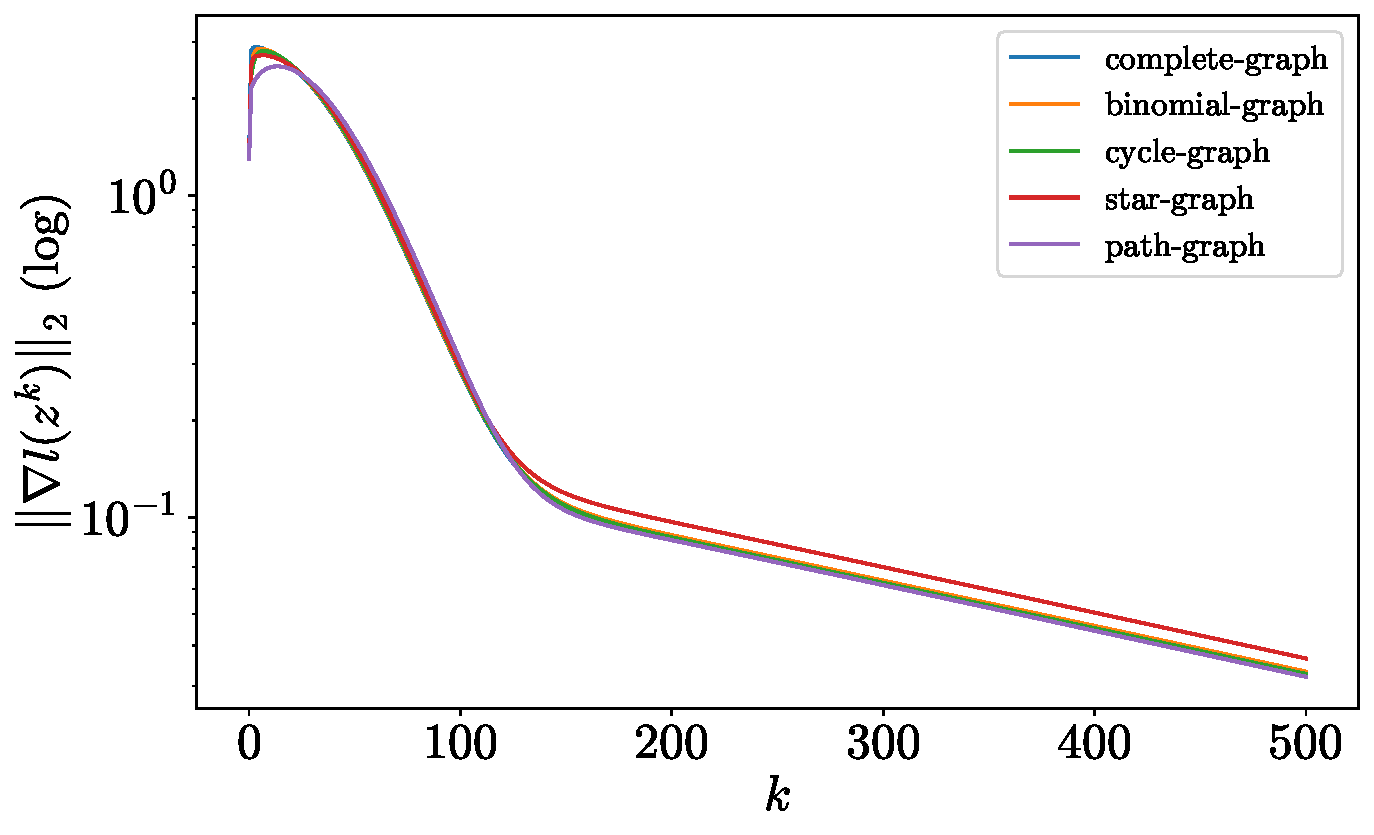
\includegraphics[width=\linewidth]{./figs/tracking/gradient_5_1_2_500.pdf} 
            \caption{Gradient norm evolution}
      \end{subfigure}
      \caption{Configuration with $5$ robots and $1$ target}
\end{figure}

\begin{figure}[H]
      \centering
      \begin{subfigure}[t]{0.49\textwidth}
            \centering
            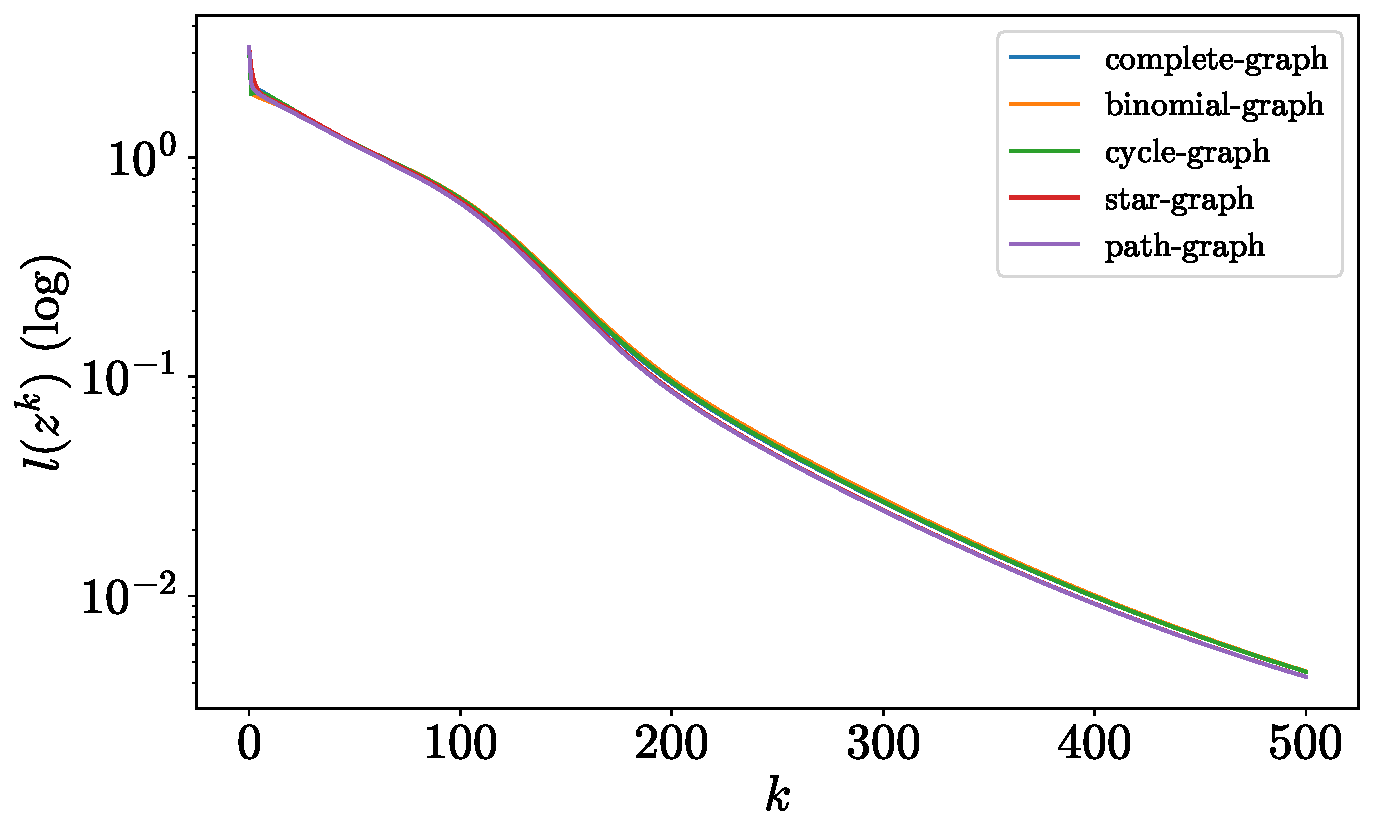
\includegraphics[width=\linewidth]{./figs/tracking/loss_5_3_2_500.pdf} 
            \caption{Loss evolution}
      \end{subfigure}
      \hfill
      \begin{subfigure}[t]{0.49\textwidth}
            \centering
            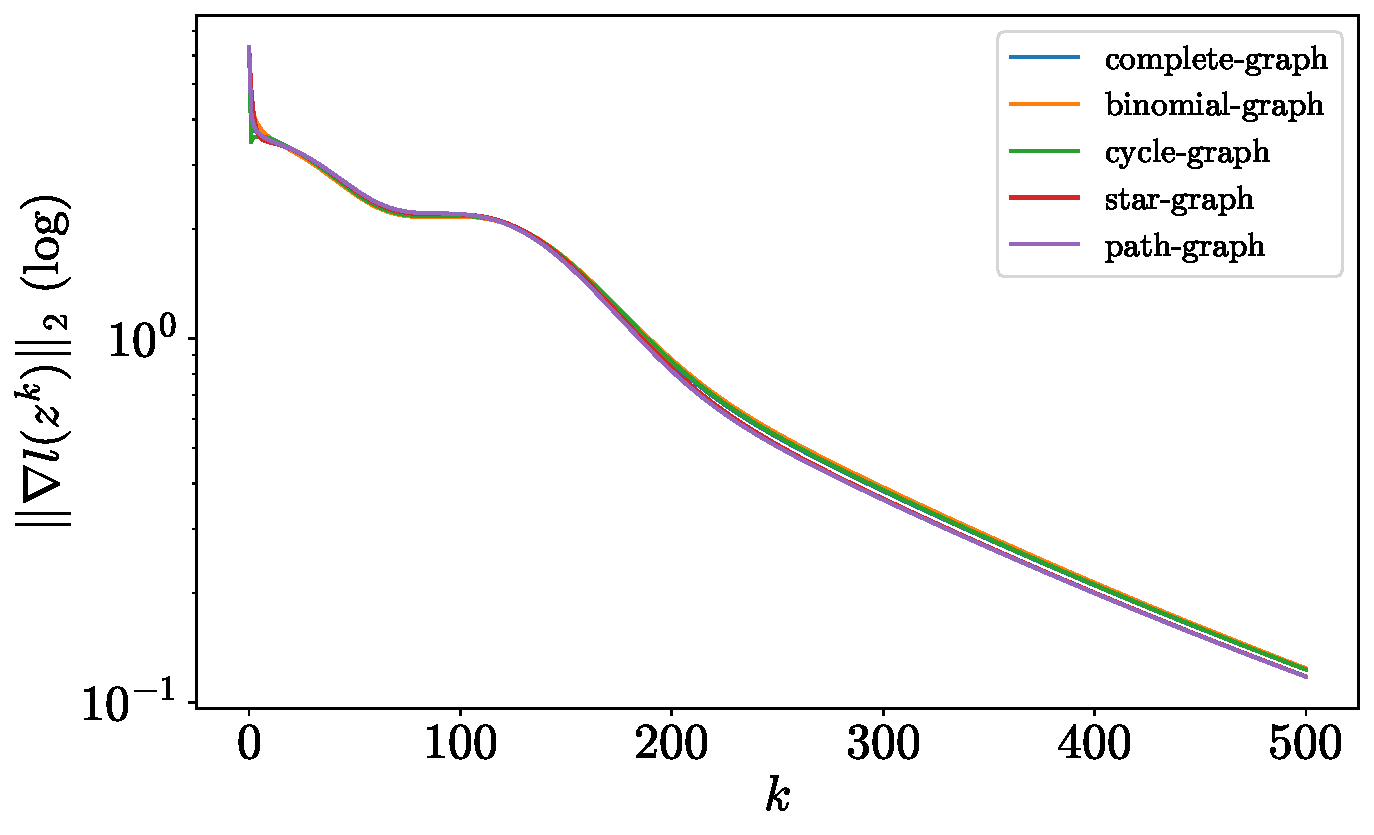
\includegraphics[width=\linewidth]{./figs/tracking/gradient_5_3_2_500.pdf} 
            \caption{Gradient norm evolution}
      \end{subfigure}
      \caption{Configuration with $5$ robots and $3$ targets}
\end{figure}

\begin{figure}[H]
      \centering
      \begin{subfigure}[t]{0.49\textwidth}
            \centering
            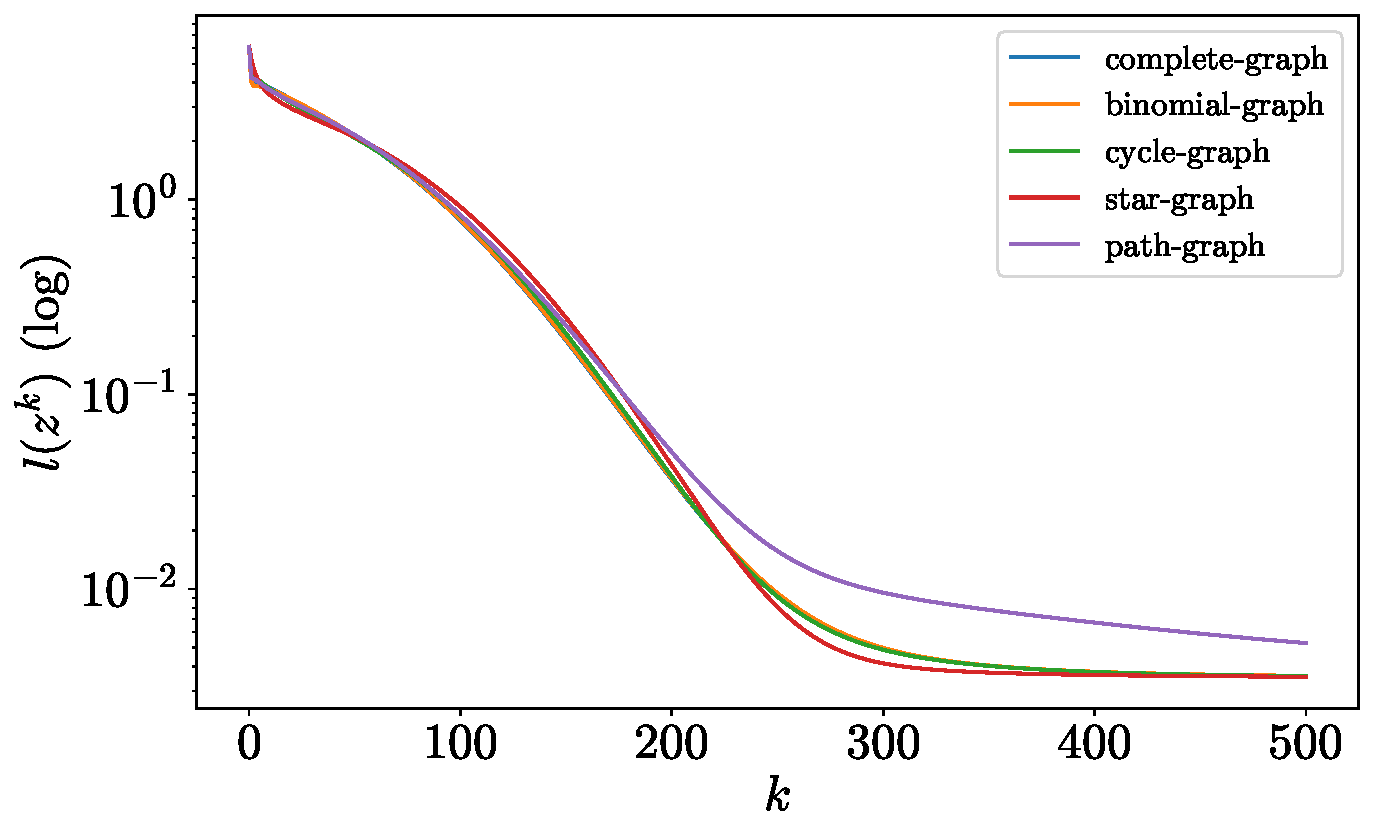
\includegraphics[width=\linewidth]{./figs/tracking/loss_15_3_2_500.pdf} 
            \caption{Loss evolution}
      \end{subfigure}
      \hfill
      \begin{subfigure}[t]{0.49\textwidth}
            \centering
            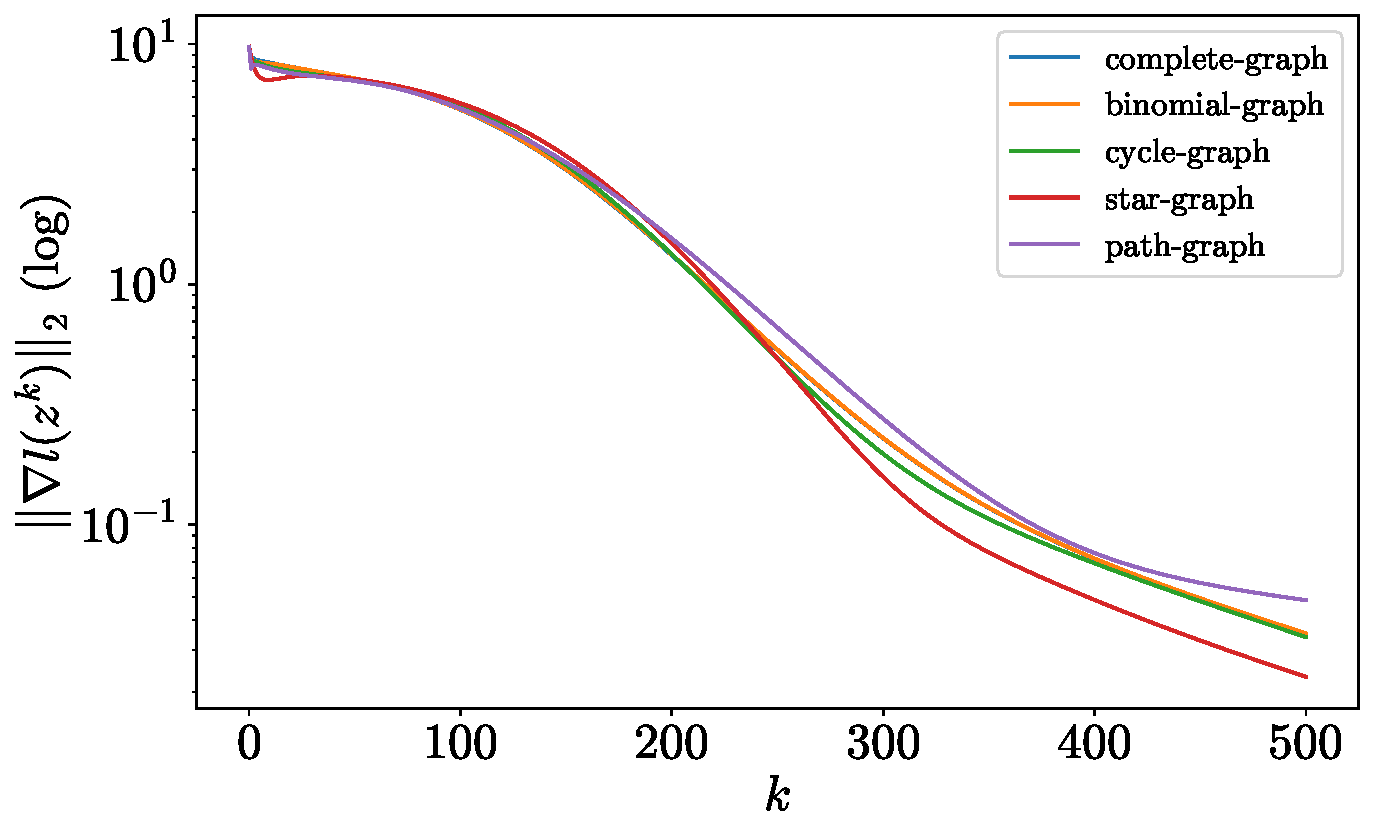
\includegraphics[width=\linewidth]{./figs/tracking/gradient_15_3_2_500.pdf} 
            \caption{Gradient norm evolution}
      \end{subfigure}
      \caption{Configuration with $15$ robots and $3$ targets}
\end{figure}



\subsection{Comparison with centralized gradient}

\begin{figure}[H]
      \centering
      \begin{subfigure}[t]{0.49\textwidth}
            \centering
            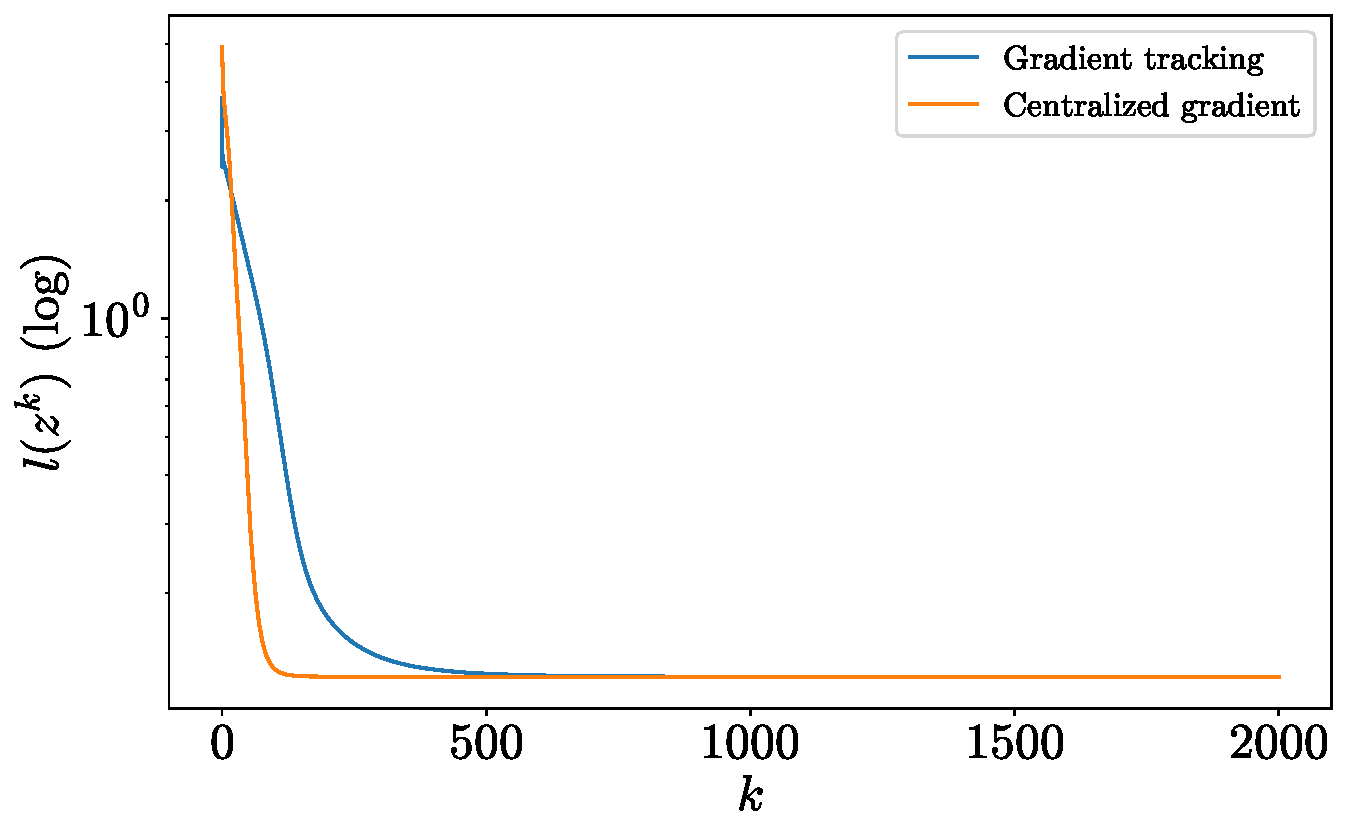
\includegraphics[width=\linewidth]{./figs/tracking/loss_centralized_5_3_2_2000.pdf} 
            \caption{Loss evolution}
      \end{subfigure}
      \hfill
      \begin{subfigure}[t]{0.49\textwidth}
            \centering
            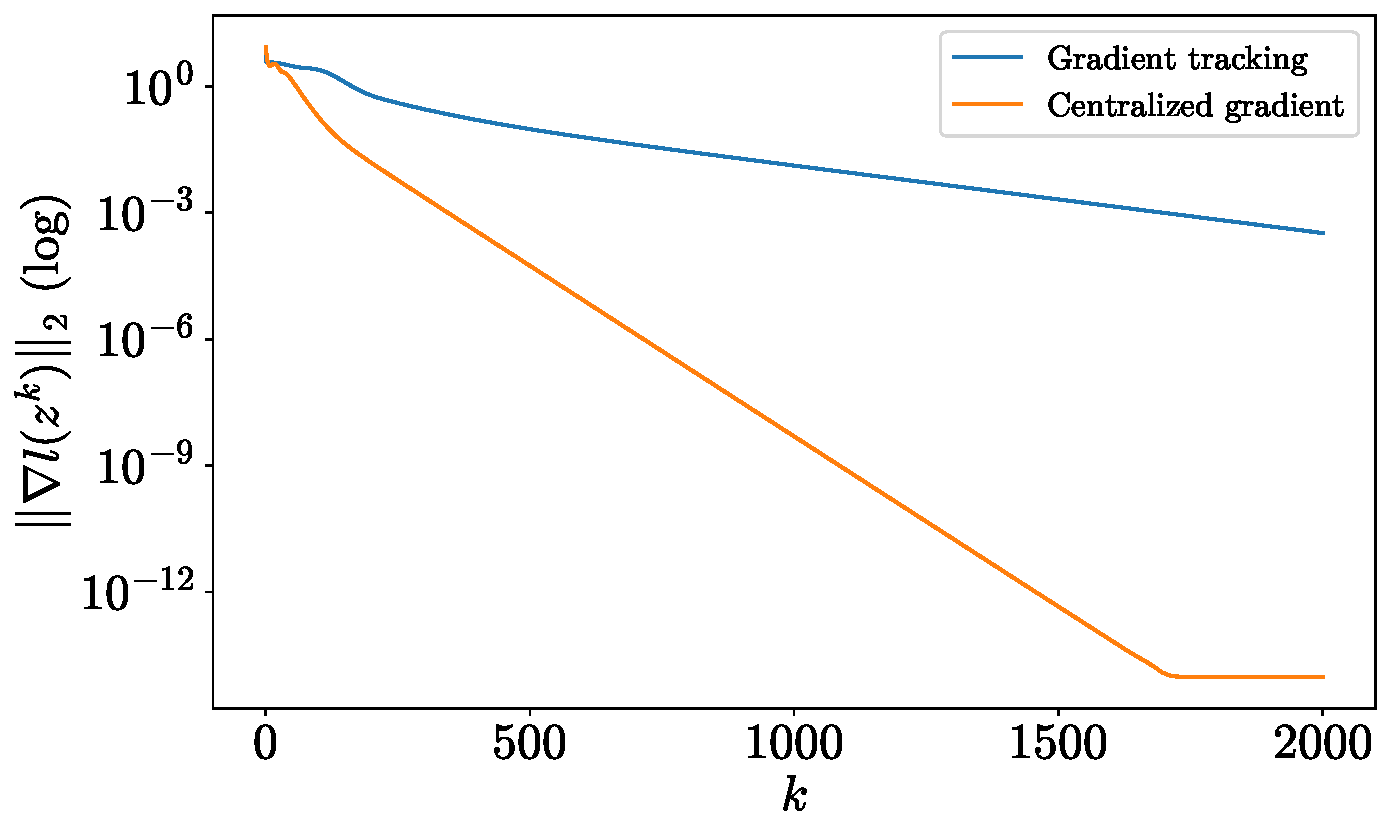
\includegraphics[width=\linewidth]{./figs/tracking/gradient_centralized_5_3_2_2000.pdf} 
            \caption{Gradient norm evolution}
      \end{subfigure}
      \caption{Configuration with $5$ robots and $3$ targets with centralized gradient}
\end{figure}


\subsection{Different noises}



\chapter{Aggregative Optimization for Multi-Robot Systems}





\chapter*{Conclusions}
\addcontentsline{toc}{chapter}{Conclusions} 



\bibliography{bibfile}{}
\bibliographystyle{plain}
\addcontentsline{toc}{chapter}{Bibliography}


\end{document}